\documentclass[11pt,conference,a4paper,onecolumn,romanappendices]{IEEEtran}
\usepackage[utf8]{inputenc}
\usepackage[english]{babel}
\usepackage{verbatim}
\usepackage{graphicx}
\usepackage{wrapfig}
\author{Lucas Colantuono, Lucas Kummer, Shanan Lynch, Samuel Sedlmeir}

\title{IoT Trace Analysis}
\date{\today}
\markboth{Improving local transports by analysing taxi meta data}{}

\author{\IEEEauthorblockN{Lucas Colantuono}
\IEEEauthorblockA{INSA Lyon \\
lucas.colantuono@insa-lyon.fr}
\and
\IEEEauthorblockN{Lucas Kummer}
\IEEEauthorblockA{INSA Lyon\\
lucas.kummer@insa-lyon.fr}
\and
\IEEEauthorblockN{Shanan Lynch}
\IEEEauthorblockA{INSA Lyon\\
shanan.lynch@insa-lyon.fr}
\and
\IEEEauthorblockN{Samuel Sedlmeir}
\IEEEauthorblockA{INSA Lyon\\
S.Sedlmeir@campus.lmu.de}}

\begin{document}

\maketitle

\tableofcontents
\newpage

\begin{abstract}
 
\end{abstract}

\section{Introduction}
\label{sec:Introduction}

\section{Related work}
There are several different articles, that analyse the same or smiliar datasets. \\
The first one, "A Metropolitan Taxi Mobility Model from Real GPS Traces", published in 2012, analysed the Taxi GPS traces from Shanghai in order to develop a model that helps understanding the needs of vehicular ad hoc networks for example. Therefore the authors computed several metrics, e.g. the turn probability at all the road crossing, implemented a map-matching algorithm and considered macro- and microscopic travel patterns. Their so called "META" model shows a higher accuracy than all other models at this time. \cite{meta} \\
Another article, "SCRAM: A Sharing Considered Route Assignment Mechanism for Fair Taxi Route Recommendations", about the same data set aimed to find an algorithm, that allows fair route sharing for every competing taxi driver. One of its goals is to not lose efficiency and a driving cost per customer as low as possible, so that it offers adavantages for the driver and the customer equally. This requires a complex evaluation algorithm that considers several prinicples which are respected my the assignment mechanism. \cite{scram}
\section{Data consistency}
The first task is to check and improve the consistency of the provided data, so that we are able to compute our chosen metric accurately. \\
At the beginning we have to filter all impossible values of the variables we're operating on. For example, our R script removes all entries with a negative speed value or timestamps outside of the interval in which these data have been collected.  Apparently the trace files only contain consistent data sets as our script has not detected and removed a single error. \\
Furthermore, there are two more types of errors that have to be considered: Checking the geographical consistency and filtering gaps in the traces.
\subsection{Geographical consistency}
\begin{wrapfigure}{r}{0.5\textwidth}
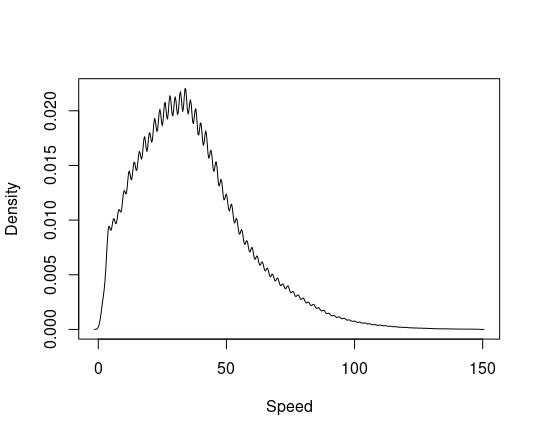
\includegraphics[scale=0.67]{speed.png}
\caption{\label{fig:speed}Adapted speed distribution without zero values}
\end{wrapfigure}
In the next step we analysed several statistical metrics concerning the speed variable which showed that there is a wide spectrum of different values, with some outliers bigger than 200 km/h, which does not make any sense in a city centre and is probably an error. That's why we decided to cut off all the entries with a speed higher than three times the interquartile range. As you can see in figure \ref{fig:speed} the speed distribution is skewed right with a single maximum. That justifies our decision, because we don't lose relevant data entries, when we choose our cut-off speed value. On the other hand side, just performing a coordinate cut is not sufficient: it changes the speed distribution slightly, e.g. we lost some data entries on the street towards one of the airports by removing all the points with a speed higher than 80 km/h. However, it does not remove all error entries. \\

The data has still to be filtered by the coordinates. As we decided to focus on the city centre, we only keep those entries in our dataset that have a longitude between 121.38 and 121.57 and a latitude between 31.15 und 31.32. In figure \ref{fig:borders} you can see our chosen borders on a map with a random sample of 100.000 points.  After restricting the data to this area, we observed a change in the distribution of the speed values as well: In general, the mean slightly decreases whilst the median is increasing strongly. As we have a right skewed distribution, we eliminate higher values with this procedure, which is the result of the fact that some streets outside don't have a low speed limit and make it necessary to perfom this cut-off. \\
\begin{figure}[h]
\centering
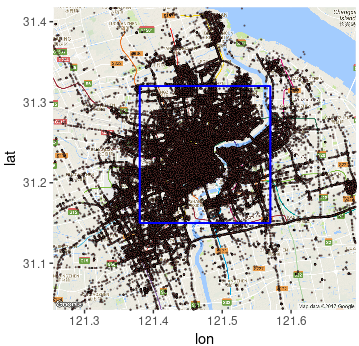
\includegraphics[scale=1]{borders.png}
\caption{\label{fig:borders}Borders of the city center}
\end{figure}
\subsection{Gap filtering}
After this procedure we are already able to plot a schematic map of Shanghai, although our dataset still contains data to be filtered. We make use of Python to find those taxi traces with a time gap between two data entries. This gap could either be a result of a data transmission error or an indicator for the beginning of a new taxi trip.\\
To define these trips in the Python code we had to choose a time gap that was appropriate for this data. So to define a trip we said that if a time gap between two data was bigger than 600 seconds or smaller than -600 seconds that it would be separated and be a new trip.\\
The reason we chose this time range was so that for future analyses of these trips we felt that this time range would keep our results consistent and more accurate. Each of these trips would be given random colours to discern one from another if we decided to plot all of these trips like in the example given. As you can see there are many trips that have been plotted and to the eye these trips seem to be valid as well. \\
\begin{wrapfigure}{r}{0.55\textwidth}
\centering
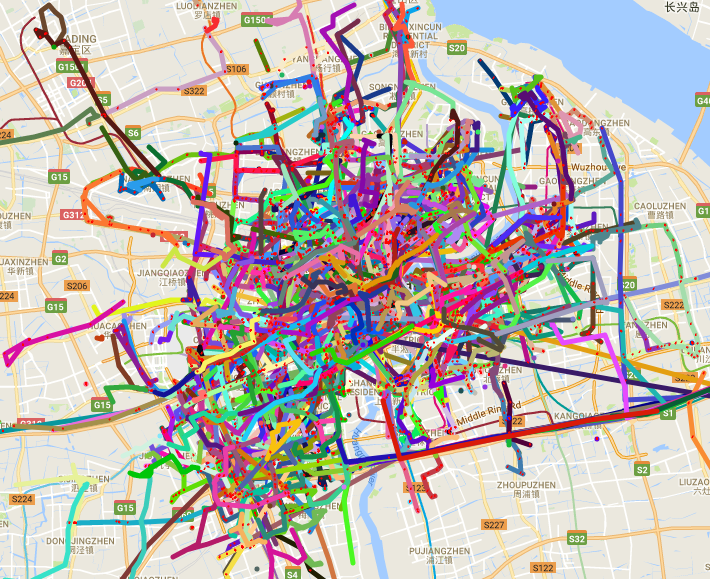
\includegraphics[scale=0.35]{plotalltrips.png}
\caption{\label{fig:plotalltrips}All calculated trips}
\end{wrapfigure}
\section{Analysis}
\section{Results}
\section{Summary}

\newpage
\bibliography{biblio}
\bibliographystyle{IEEEtran}

\end{document}
